\documentclass{article}
\usepackage[utf8]{inputenc}
\usepackage[T1]{fontenc}
\usepackage[russian]{babel}
\usepackage{tikz}
\usepackage{graphicx}
\usepackage{titlesec}
\usepackage{amsfonts}
\usepackage{amsmath}
\usepackage[left=2cm,right=2cm,
    top=2cm,bottom=2cm,bindingoffset=0cm]{geometry}
\renewcommand{\thesection}{\arabic{section}}
\titleformat{\section}{\large\bfseries}{\thesection}{1em}{}
\title{Интегрирование}
\author{Каренин Константин Витальевич}
\date{02.04.2024}
\begin{document}

\begin{titlepage}
    \centering
    \vspace*{0.5 cm}
    
    \textsc{\LARGE \textbf{Математический анализ}}
    \vspace{1.5cm}
    
    \rule{\linewidth}{0.2 mm} \\[0.4 cm]
    { \huge \bfseries Интегрирование}
    \rule{\linewidth}{0.2 mm} \\[1.5 cm]
    
    \Large Выполнили: \\
    Каренин Константин \\
    Темиров Тимур \\
    Гонин Сергей \\
    Малышева Алиса \\
    
    \vspace{0.5cm}
    
    Группа: М3104
    
    \vspace{0.5cm}
    
    Преподаватель: Сарычев Павел
    
    \vspace{0.5cm}
    
    Университет ИТМО
    
    \vfill

    
\includegraphics[height=70px]{logo.jpg}
    
    2.04.2024
    
\end{titlepage}

\setcounter{page}{2}

% task 1
\newpage
    \section{
    \begin{equation*}
    g(x) = 
    \begin{cases}
        e^x-e, \;x < 0 \\
        \ln{(3x+1)}, \;0 \leq x \leq 1 \\
        e^{-x}, \;x > 0 \\
    \end{cases}
    \end{equation*}
    }
    \subsection{Найдите такую непрерывную функцию $f (x)$, что $f'(x) = g(x)$}
    Пусть $f(x)$ - первообразная $g(x)$\\
    \begin{equation*}
    f(x) = 
    \begin{cases}
        e^x-ex + C_1, \;x < 0 \\
        (x+\frac{1}{3})\ln{(3x+1)} - (x + \frac{1}{3}) + C_2, \;0 \leq x \leq 1 \\
        -e^{-x} + C_3, \;x > 0 \\
    \end{cases}
    \end{equation*}
    Чтобы $f(x)$ была непрерывна возьмём $C_1=-1 , C_2= \frac{1}{3} , C_3= \frac{8}{3} \ln{2} - 1 + \frac{1}{\text{e}}$

    \subsection{Графики функций}
    \begin{equation*}
       g(x) 
    \end{equation*}
    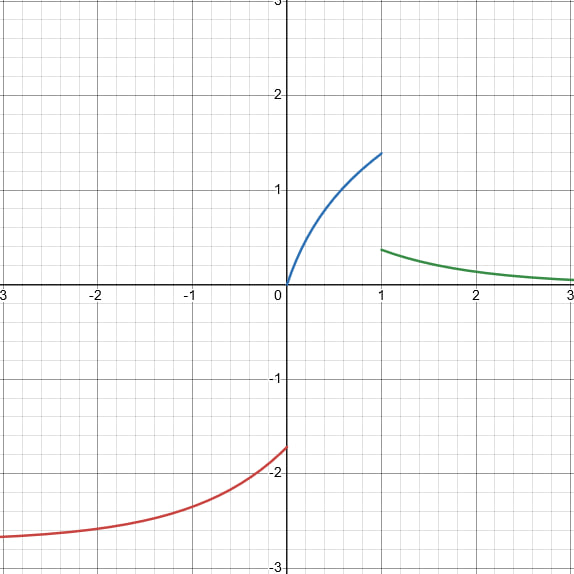
\includegraphics[height=300px]{g(x).jpg}\newpage
    \begin{equation*}
        f(x)
    \end{equation*}
    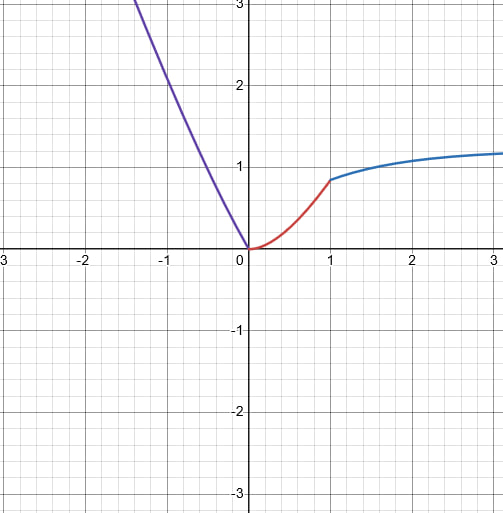
\includegraphics[height=300px]{f(x).jpg}
    \subsection{Анализ графиков}
    График $f$ имеет существенные отличия от $g$, поскольку в первой части добавляется $x$ при $e$, во второй изменяется первообразная логорифма, а в третьей график отражается относительно $Ox$. Графики не имеют определённого вида, поэтому вывод о зависимости сделать невозможно        

    
% task 2
\newpage
    \section{
    \begin{equation*}
    I_p = \int_{0}^3 \frac{px \, dx}{(9-x^2)^{p^2-p-7}}
    \end{equation*}
    }
    \begin{equation*}
    \int\frac{px \, dx}{(g-x^{2})^{p^2-p-7}} = p\int x(9-x^{2})^{-p^2+p+7} \, dx = -\frac{p(9-x^{2})^{-p^2+p+8}}{2(-p^{2}+p+8)} + C
    \end{equation*}
    Поскольку $f(x)= \frac{px \, dx}{(9-x^2)^{p^2-p-7}}$ неограничена на $[0 , 3]$, то $\int_{0}^3 f(x) \, dx$ - несобственный \\
    При выражение=0 знаменатель будет равен единице, тогда:\\
    $p = \frac{1 \pm \sqrt{29}}{2}$\\
    При $p = \frac{1 \pm \sqrt{29}}{2} \quad I_p$ - собственный\\
    При $p = 0 \quad I_p$ - несобственный сходящийся\\
    $p^2 - p - 8 > 0 \quad I_p$ - несобственный расходящийся\\
    $p \in (- \infty ; \frac{1 - \sqrt{65}}{2}] \cup [\frac{1 + \sqrt{65}}{2} ; + \infty) \quad - I_p$ - несобственный расходящийся\\
    $p \in (\frac{1 - \sqrt{65}}{2} ; \frac{1 + \sqrt{65}}{2}] \backslash \{\frac{1 \pm \sqrt{29}}{2}\} \quad - I_p$ - несобственный сходящийся\\
    \subsection{Ответ}
    При $p = \frac{1 \pm \sqrt{29}}{2} \quad I_p$ - собственный\\
    $p \in (- \infty ; \frac{1 - \sqrt{65}}{2}] \cup [\frac{1 + \sqrt{65}}{2} ; + \infty) \quad - I_p$ - несобственный расходящийся\\
    $p \in (\frac{1 - \sqrt{65}}{2} ; \frac{1 + \sqrt{65}}{2}] \backslash \{\frac{1 \pm \sqrt{29}}{2}\} \quad - I_p$ - несобственный сходящийся
    

% task 3
\newpage
    \section{
    \begin{equation*}
    f(x) = \frac{x^4-4x^3+6x^2-4x+16}{3(x-2)^3}    
    \end{equation*}
    }
    $f(x) = \frac{x^4-4x^3+6x^2-4x+16}{3(x-2)^3} = \frac{1}{3}x -\frac{1}{3} + \frac{5}{(x-1)^3}$
    \subsection{Найдем наклонную асимптоту}
    $y = kx + b$ \\
    $k = \lim\limits_{x \to \infty} \frac{f(x)}{x} = \lim\limits_{x \to \infty} \frac{\frac{1}{3}x-\frac{1}{3}+\frac{5}{(x-1)^3}}{x} = \frac{1}{3}$ \\
    $b = \lim\limits_{x \to \infty} (f(x)-kx) = \lim\limits_{x \to \infty} (\frac{1}{3}x-\frac{1}{3}+\frac{5}{(x-1)^3}-\frac{1}{3}x) = -\frac{1}{3}$ \\
    $y = \frac{x}{3} - \frac{1}{3}$ \\
    $x = 1$ - точка разрыва второго ряда, вертикальная ассимптота 
    \subsection{График}
    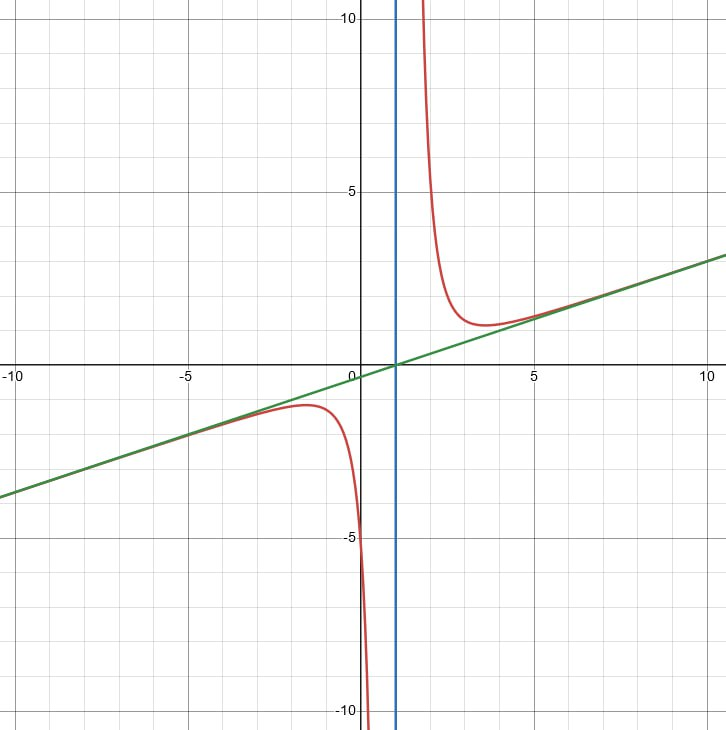
\includegraphics[height=300px]{график3.jpg}
    \subsection{Интегрирование}
    \begin{equation*}
        \int_1^{+\infty} (\frac{x}{3}-\frac{1}{3}+\frac{5}{(x-1)^3}-(\frac{x}{3}-\frac{1}{3}) )\, dx = 
        \int_1^2 \frac{5}{(x-1)^3} \, dx + \int_2^{+\infty} \frac{5}{(x-1)^3} \, dx = 
        \lim\limits_{a \to 1+} \int_a^2 \frac{5}{(x-1)^3} \, dx + \lim\limits_{a \to +\infty} \int_2^{+\infty} \frac{5}{(x-1)^3} \, dx =
    \end{equation*}
    \begin{equation*}
        = \lim\limits_{a \to 1+} (-\frac{5}{2}+\frac{5}{2(a-1)^2}) + \lim\limits_{a \to +\infty} (-\frac{5}{2(a-1)^2} + \frac{5}{2}) = + \infty \; \Rightarrow \text{интеграл расходящийся}
    \end{equation*}
     Из расходящегося несобственного интеграла следует, что площадь невозможно определить
    



% task 4
\newpage
    \section{Вычислите работу, которую нужно затратить на выкачивание воды из резервуара, представляющего из себя
правильную четырёхугольную пирамиду, обращённой вершиной вниз. Сторона основания пирамиды 2 м, высота
– 6 м.}
    \subsection{Графическая иллюстрация}
    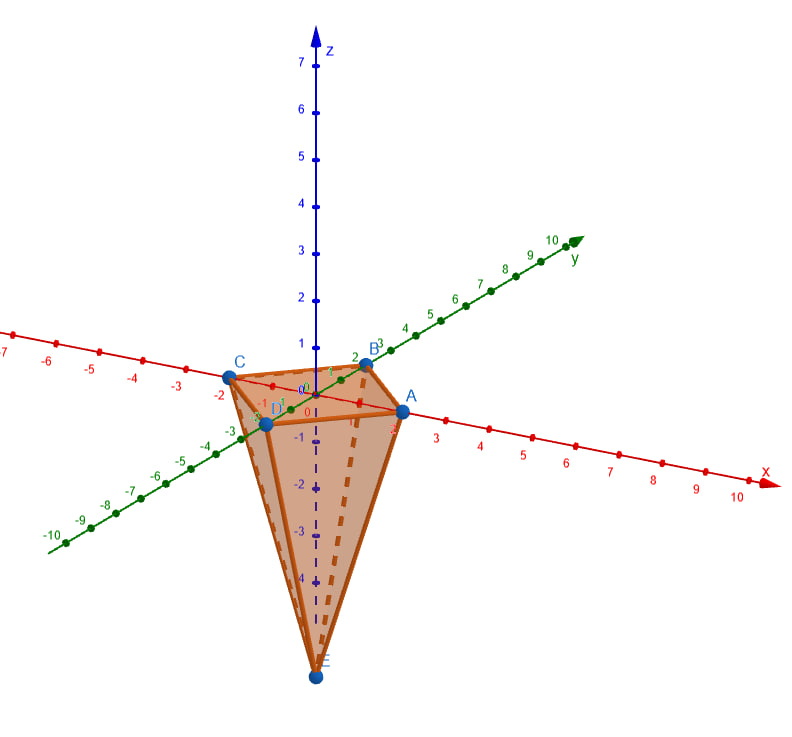
\includegraphics[height=300px]{график41.jpg}
    \subsection{Математичская модель}
Для решения этой задачи мы можем использовать интеграл для вычисления
работы. Рассмотрим правильную четырёхугольную пирамиду, обращённую
вершиной вниз, с основанием в форме квадрата.\\
Введем обозначения: \\
$a$ - сторона квадрата основания пирамиды (в данном случае $a=2 \, \text{м}$).\\
$S$ - площадь основания пирамиды (квадрата), равная $2^2 = 4 \, \text{м}^2$\\
$H$ - высота пирамиды (в данном случае равная 6 м).\\
$h$ - это расстояние от уровня воды до основания пирамиды\\
Также нам понадобятся физические константы:\\
$\rho$ - плотность воды, которая в данном случае равна $1000 \, \frac{\text{кг}}{\text{м}^3}$\\
$g$ - ускорение свободного падения, принятое за $9.8 \, \frac{\text{м}}{\text{с}^2}$ \\
Составим формулу:\\
Чтобы выкачать воду из бака, нужно совершить работу А, чтобы преодолеть
силу тяжести, то есть $A = Fт = mgh$\\
Неизвестную массу распишем как $m = \rho V$\\
Далее объем V воды, который мы поднимаем, можно выразить как
произведение площади основания пирамиды $S$ на ее высоту $h$. Это даёт нам
$V=Sh$\\
Заметим, что для каждого слоя воды, находящегося на определенной высоте
$h$ от основания пирамиды, работа, совершаемая чтобы его выкачать, будет
отличаться ввиду изменения объёма слоя, и высоты на которую необходимо
поднять эту воду при выкачивании.\\
Чтобы учесть то, что с изменением высоты меняется объем воды внутри
пирамиды, мы должны представить весь поднимаемый объем как множество
слоев воды бесконечно малого объема (а именно, бесконечно малой высоты
слоя с заданной площадью его основания).\\
Рассмотрим некоторый слой воды, высота которого $dh$, при этом его площадь
основания равна площади поперечного сечения пирамиды плоскостью,
параллельной $Оху$ на расстоянии $h$ от основания пирамиды (само сечение
является квадратом):\\
Найдем зависимость площади сечения $S$ от $h$, для этого рассмотрим рисунок:\\
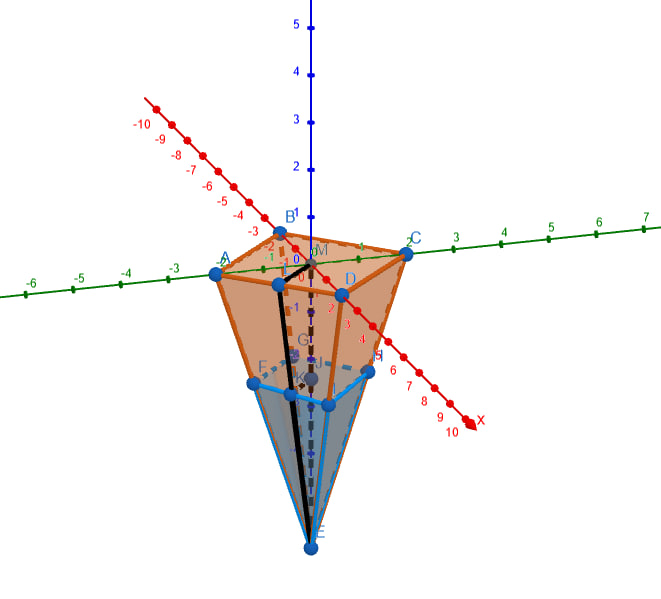
\includegraphics[height=300px]{график42.jpg} \\
На рисунке треугольники $ЕML$ и $EJK$ (выделены черным) подобны. Пусть $k = \frac{h}{H}$ - коэффициент подобия. Если в большой и маленькой пирамидах линейные
величины подобны с коэффициентом $k$ (в том числе стороны оснований $AD$ и
$FI$) то площади соотносятся как $\frac{S_{\text{сеч}}}{S_{\text{осн}}} = \frac{FI^2}{AD^2} = k^2 = (\frac{h}{H})^2$\\
Отсюда
$S(h) = S_{\text{сеч}} = k^2 S_{\text{осн}} = \frac{h^2 S_{\text{осн}}}{H^2} = \frac{h^2 a^2}{H^2}$\\
Чтобы найти объем такого слоя умножим произведение площади основания
$S(h)$ на бесконечно малую высоту $dh$, что дает нам формулу $dV=S(h)dh$ для
правильного вычисления объема.\\
Масса слоя воды бесконечно малого объема:\\
Мы знаем, что масса $m$ зависит от плотности $\rho$ и объема $V$ как $m=\rho V$.\\
Подставив сюда формулу для $V$, получаем $dm = \rho dV = \rho S(h)dh$.\\
Работа, необходимая для подъема слоя воды высотой $dh$:\\
$dA=g(H - h)dm=g(H - h)\rho S(h)dh$\\
Теперь мы можем интегрировать $dA$ от 0 до $H$, чтобы найти общую работу $A$,
затрачиваемую на выкачивание всей воды из резервуара.
    \subsection{Аналитическое решение}
    Чтобы найти работу $A$, проинтегрируем $dA$ от $0$ до $H$:\\
    $A = \int_0^H g(H-h)\rho S(h) \, dh$\\
    Преобразуем и решим интеграл:\\
    $A &= g\rho \int_0^H (H-h)S(h) \, dh$ \\
    $= g\rho \int_0^H (H-h)\left(\frac{h^2a^2}{H^2}\right) \, dh$ \\
    Подставляем известные значения: по условию а = 2 м, Н = 6 м\\
    $A= g\rho \int_0^6 (6-h)\left(\frac{h^2(2\text{ м})^2}{6^2}\right) \, dh$ \\
    $= g\rho \int_0^6 (6-h)\left(\frac{h^2}{9}\right) \, dh$ \\
    $= \frac{g\rho}{9} \int_0^6 (6h^2-h^3) \, dh$ \\
    $= \frac{g\rho}{9} \left(2h^3 - \frac{h^4}{4}\right) \bigg|_0^6$ \\
    $= \frac{g\rho}{9} \left(2(6^3) - \frac{6^4}{4} - 0\right)$ \\
    $= \frac{g\rho}{9} \left(2(216) - \frac{1296}{4}\right)$ \\
    $= \frac{g\rho}{9} \cdot 6^3 \cdot \left(2 - \frac{3}{2}\right)$ \\
    $= \frac{g\rho}{9} \cdot 6^3 \cdot \left(\frac{1}{2}\right)$\\
    Подставляем константные значения:\\
    $g = 9.8 \, \frac{\text{м}}{\text{с}^2}$ \\
    $\rho = 1000 \, \frac{\text{кг}}{\text{м}^3}$ \\
    $A = \frac{9.8 \times 1000 \times (6^3)}{9 \times 2} = \frac{9.8 \times 1000 \times 216}{18} = 117600 \, \text{Дж}$


    
% evaluation paper
\newpage
\[
\renewcommand{\arraystretch}{2}
\begin{tabular}{| c | c |}
 \hline
    \hugeУчастник & \hugeВклад в \% \\
 \hline
    \hugeКаренин Константин & \huge25 \\
 \hline
    \hugeГонин Сергей & \huge25 \\
 \hline
    \hugeТемиров Тимур & \huge25 \\
 \hline
    \hugeМалышева Алиса & \huge25 \\
 \hline
\end{tabular}
\]
\end{document}